\documentclass{beamer}
\usetheme{Warsaw}
\usecolortheme{seahorse}
\usepackage{amsmath}
\usepackage{amsfonts}
\usepackage{amssymb}
%\usepackage{CJKutf8}
\title{Introduction to Fourier transform and signal analysis}
\author{\texorpdfstring{Zong-han, Xie\newline\url{icbm0926@gmail.com}}{Zong-han, Xie}}
\begin{document}
%\begin{CJK}{UTF8}{cwmc}
\begin{frame}
\titlepage
\end{frame}
\begin{frame}[label=licensepage]
\frametitle{License of this document}
Introduction to Fourier Transform and Signal Analysis by Zong-han, Xie (\href{icbm0926@gmail.com}{icbm0926@gmail.com}) is licensed under a Creative Commons Attribution-NonCommercial 4.0 International License. \newline
\begin{center}
\includegraphics[scale=1]{by-nc-sa.eps}
\end{center}
\end{frame}
\AtBeginSection[]
{
  \begin{frame}
    \frametitle{Outline}
    \tableofcontents[currentsection]
  \end{frame}
}
\section{Continuous Fourier transform}
\begin{frame}
\frametitle{Orthogonal condition}
\begin{itemize}
\item Any two vectors $\mathbf{a}$, $\mathbf{b}$ satisfied the following condition are mutually orthogonal. \newline
\begin{eqnarray}
\mathbf{a}^* \cdot \mathbf{b} = 0
\label{eq:ortho_vec}
\end{eqnarray}
\item Any two functions $a(x)$, $b(x)$ satisfied the following condition are mutually orthogonal. \newline
\begin{eqnarray}
\int{a^*(x)} \cdot {b(x)} dx = 0
\label{eq:ortho_func}
\end{eqnarray}
\item * means complex conjugate. \newline
\end{itemize}
\end{frame}
\begin{frame}
\frametitle{Complete and orthogonal basis}
\begin{itemize}
\item $\cos nx $ and $\sin mx$ are mutually orthogonal in which n and m are integers.
\begin{eqnarray}
\int_{-\pi}^{\pi}{\cos nx} \cdot {\sin mx} dx = 0 \nonumber \\
\int_{-\pi}^{\pi}{\cos nx} \cdot {\cos mx} dx = \pi\delta_{nm} \nonumber \\
\int_{-\pi}^{\pi}{\sin nx} \cdot {\sin mx} dx = \pi\delta_{nm}
\end{eqnarray}
\item $\delta_{nm} $ is Dirac-delta symbol. It means $\delta_{nn} = 1$ and $\delta_{nm} = 0$ when $n \neq m$.
\end{itemize}
\end{frame}
\begin{frame}
\frametitle{Fourier series}
Since $\cos nx $ and $\sin mx$ are mutually orthogonal, we can expand an arbitrary periodic function $f(x)$ by them. we shall have a series expansion of $f(x)$ which has $2\pi$ period.
\begin{eqnarray}
f(x)&=&a_0 + \sum_{k=1}^{\infty} \left(a_k\cos kx + b_k \sin kx\right) \nonumber \\
a_0&=&\frac{1}{2\pi}\int_{-\pi}^{\pi}f(x) dx \nonumber \\
a_k&=&\frac{1}{\pi}\int_{-\pi}^{\pi}f(x) \cos kx dx \nonumber \\
b_k&=&\frac{1}{\pi}\int_{-\pi}^{\pi}f(x) \sin kx dx
\label{eq:fseries}
\end{eqnarray}
\end{frame}
\begin{frame}
\frametitle{Fourier series}
If $f(x)$ has $L$ period instead of $2\pi$, $x$ is replaced with $\pi x /L$.
\begin{eqnarray}
f(x)&=&a_0 + \sum_{k=1}^{\infty} \left(a_k\cos \frac{2k\pi x}{L} + b_k \sin \frac{2k\pi x}{L}\right) \nonumber \\
a_0&=&\frac{1}{L}\int_{-\frac{L}{2}}^{\frac{L}{2}}f(x) dx \nonumber \\
a_k&=&\frac{2}{L}\int_{-\frac{L}{2}}^{\frac{L}{2}}f(x) \cos \frac{2k\pi x}{L} dx, k = 1,2,...\nonumber \\
b_k&=&\frac{2}{L}\int_{-\frac{L}{2}}^{\frac{L}{2}}f(x) \sin \frac{2k\pi x}{L} dx, k = 1,2,...
\label{eq:fseries_pL}
\end{eqnarray}
\end{frame}
\begin{frame}
\frametitle{Complex Fourier series}
Using Euler's formula, equation (\ref{eq:fseries}) becomes 
\begin{eqnarray}
f(x)=a_0 + \sum_{k=1}^{\infty} \left(\frac{a_k - ib_k}{2} e^{ikx} + \frac{a_k + ib_k}{2}e^{-ikx}\right) \nonumber
\end{eqnarray}
Let $c_0 \equiv a_0$, $c_k \equiv \frac{a_k - ib_k}{2}$ and $c_{-k} \equiv \frac{a_k + ib_k}{2}$, we have
\begin{eqnarray}
f(x)&=&\sum_{m=-\infty}^{\infty} c_m e^{imx} \nonumber \\
c_m&=&\frac{1}{2\pi}\int_{-\pi}^{\pi} f(x) e^{-imx} dx
\label{eq:cfseries}
\end{eqnarray}
$e^{imx}$ and $e^{inx}$ are also mutually orthogonal provided $n \neq m$ and it forms a complete set. Therfore, it can be used as orthogonal basis.\newline
\end{frame}
\begin{frame}
\frametitle{Complex Fourier series}
If $f(x)$ has $T$ period instead of $2\pi$, $x$ is replaced with $2\pi x /T$.
\begin{eqnarray}
f(x)&=&\sum_{m=-\infty}^{\infty} c_m e^{i\frac{2\pi mx}{T}} \nonumber \\
c_m&=&\frac{1}{T}\int_{-\frac{T}{2}}^{\frac{T}{2}} f(x) e^{-i\frac{2\pi mx}{T}} dx, m = 0,1,2...
\label{eq:cfseries_pT}
\end{eqnarray}
\end{frame}
\begin{frame}
\frametitle{Fourier Series of step function}
$f(x)$ is a periodic function with $2\pi$ period and it's defined as follows.
\begin{eqnarray}
f(x)&=& 0, -\pi < x < 0 \nonumber \\
f(x)&=& h, 0 < x < \pi
\label{eq:stepfunc}
\end{eqnarray}
Fourier series of $f(x)$ is
\begin{eqnarray}
f(x)= \frac{h}{2} + \frac{2h}{\pi} \left( \frac{\sin x}{1} + \frac{\sin 3x}{3} + \frac{\sin 5x}{5} + ...\right)
\label{eq:stepfunc_ft}
\end{eqnarray}
$f(x)$ is piecewise continuous within the periodic region. Fourier series of $f(x)$ converges at speed of $1/n$.
\end{frame}
\begin{frame}
\frametitle{Fourier series of step function}
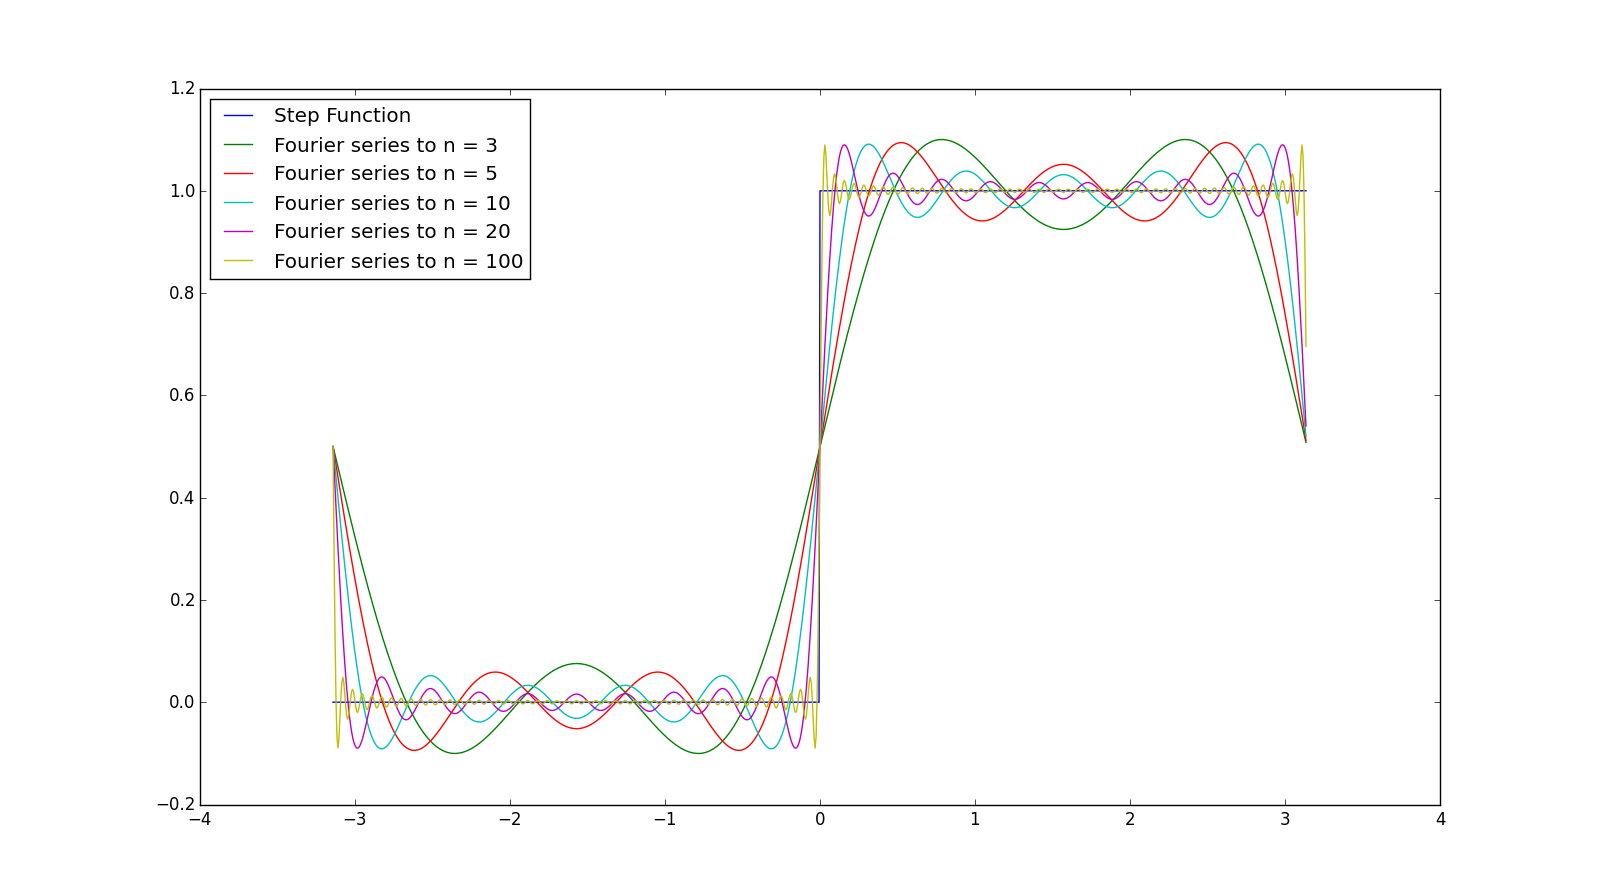
\includegraphics[scale=0.3]{step.png}
\end{frame}
\begin{frame}
\frametitle{Fourier series of saw tooth function}
$f(x)$ is a periodic function with $2\pi$ period and it's defined as follows.
\begin{eqnarray}
f(x)&=& -x, -\pi < x < 0 \nonumber \\
f(x)&=& x, 0 < x < \pi
\label{eq:sawfunc}
\end{eqnarray}
Fourier series of $f(x)$ is
\begin{eqnarray}
f(x)= \frac{\pi}{2} - \frac{4}{\pi} \sum_{n=1,3,5...} \left( \frac{\cos nx}{n^2} \right)
\label{eq:sawfunc_ft}
\end{eqnarray}
$f(x)$ is continuous and its derivative is piecewise continuous within the periodic region. Fourier series of $f(x)$ converges at speed of $1/n^2$.
\end{frame}
\begin{frame}
\frametitle{Fourier series of saw tooth function}
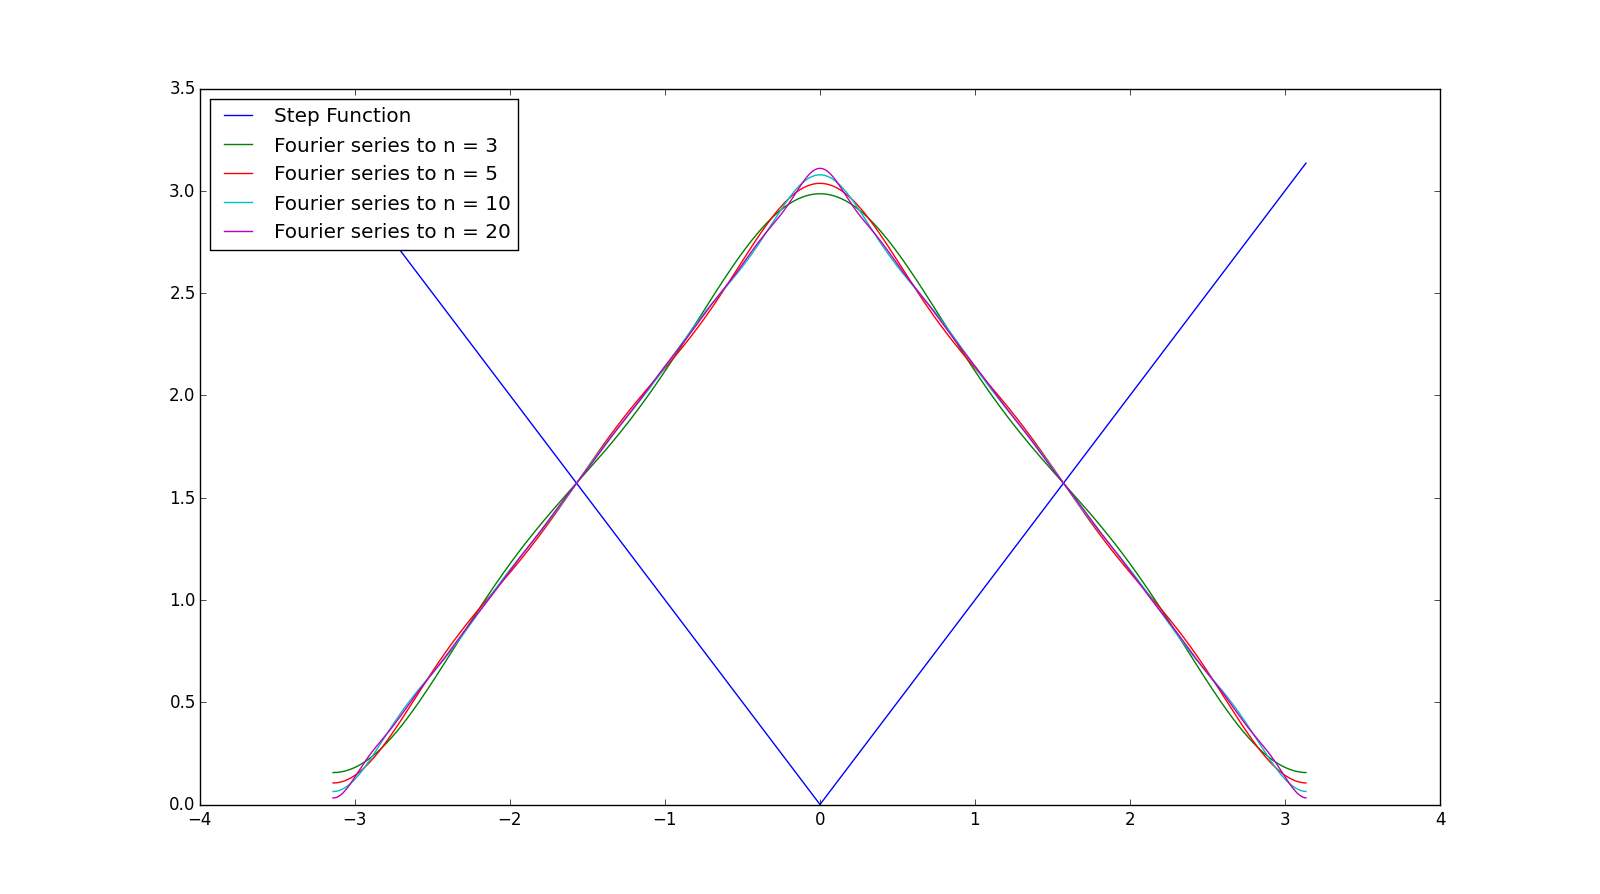
\includegraphics[scale=0.3]{sawtooth.png}
\end{frame}
\begin{frame}
\frametitle{Fourier series of full wave rectifier}
$f(t)$ is a periodic function with $2\pi$ period and it's defined as follows.
\begin{eqnarray}
f(t)&=& -\sin {\omega t}, -\pi < t < 0 \nonumber \\
f(t)&=& \sin {\omega t}, 0 < t < \pi
\label{eq:fullrectifier_func}
\end{eqnarray}
Fourier series of $f(x)$ is
\begin{eqnarray}
f(t)= \frac{2}{\pi} - \frac{4}{\pi} \sum_{n=2,4,6...} \left( \frac{\cos n\omega t}{n^2 - 1} \right)
\label{eq:fullrectifier_func_ft}
\end{eqnarray}
$f(x)$ is continuous and its derivative is piecewise continuous within the periodic region. Fourier series of $f(x)$ converges at speed of $1/n^2$.
\end{frame}
\begin{frame}
\frametitle{Fourier series of full wave rectifier}
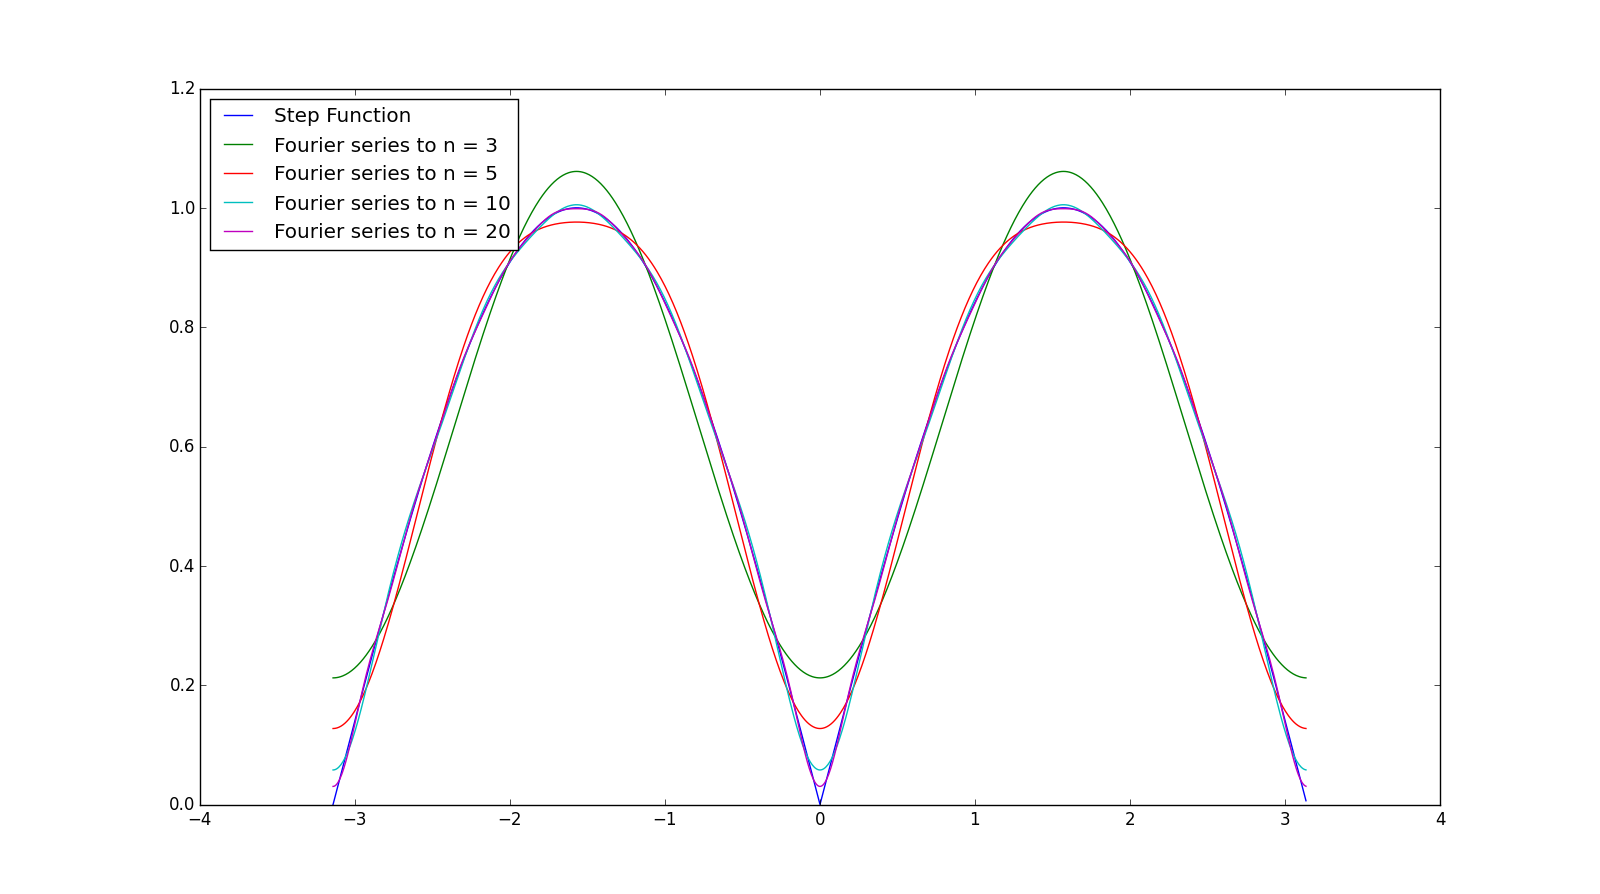
\includegraphics[scale=0.3]{fullrectifier.png}
\end{frame}
\begin{frame}
\frametitle{Fourier transform}
from Eq. \ref{eq:cfseries_pT}, we define variables $k \equiv \frac{2\pi m}{T}$, $\hat{f}(k) \equiv\frac{c_mT}{\sqrt{2\pi}}$ and $ \bigtriangleup{k} \equiv \frac{2\pi (m+1)}{T} - \frac{2\pi m}{T} = \frac{2\pi}{T}$. \newline We can have
\begin{eqnarray}
f(x)&=&\frac{1}{\sqrt{2\pi}}\sum_{m=-\infty}^{\infty} \hat{f}(k) e^{ikx} \bigtriangleup{k} \nonumber \\
\hat{f}(k)&=&\frac{1}{\sqrt{2\pi}}\int_{-\frac{T}{2}}^{\frac{T}{2}} f(x) e^{-ikx}dx\nonumber
\end{eqnarray}
\end{frame}
\begin{frame}
\frametitle{Fourier transform}
Let $T\longrightarrow\infty$
\begin{eqnarray}
f(x)&=&\frac{1}{\sqrt{2\pi}}\int_{-\infty}^{\infty} \hat{f}(k) e^{ikx} dk
\label{eq:ftransform_inv}\\
\hat{f}(k)&=&\frac{1}{\sqrt{2\pi}}\int_{-\infty}^{\infty} f(x) e^{-ikx} dx
\label{eq:ftransform}
\end{eqnarray}
Eq.\ref{eq:ftransform} is the \emph{Fourier transform} of $f(x)$ and Eq.\ref{eq:ftransform_inv} is the \emph{inverse Fourier transform} of $\hat{f}(k)$.
\end{frame}
\begin{frame}
\frametitle{Convolution theory and Parseval relation}
Considering two functions $f(x)$ and $g(x)$ with their Fourier transform $F(k)$ and $G(k)$. We define an operation
\begin{eqnarray}
f\ast g = \int_{-\infty}^{\infty}g(y)f(x-y)dy
\label{eq:convolution}
\end{eqnarray}
as the convolution of the two functions $f(x)$ and $g(x)$ over the interval $\{ -\infty \sim \infty \}$. It satisfies the following relation:
\begin{eqnarray}
f \ast g = \int_{-\infty}^{\infty}F(k)G(k) e^{ikx}dt
\label{eq:convolution_theorem}
\end{eqnarray}
It shows that convolution of two functions is the same as the inverse Fourier transform of the direct product of their Fourier transform.
\end{frame}
\begin{frame}
\frametitle{Correlation}
\end{frame}
\begin{frame}
\frametitle{Uncertainty principle}
\end{frame}
\begin{frame}
\frametitle{Fourier transform of a Gaussian function}
\end{frame}
\begin{frame}
\frametitle{Fourier transform of a Gaussian function with carrier}
\end{frame}
\begin{frame}
\frametitle{Transfer function}
\end{frame}
\section{Discrete Fourier transform}
\begin{frame}
\frametitle{From continuous to discrete Fourier transform}
\end{frame}
\begin{frame}
\frametitle{Frequency bins and nyquist frequency}
\end{frame}
\begin{frame}
\frametitle{Concept of Nyquist-Shannon frequency}
\end{frame}
\begin{frame}
\frametitle{Aliasing}
\end{frame}
\begin{frame}
\frametitle{Window functions}
\end{frame}
\begin{frame}
\frametitle{Filter}
\end{frame}
\begin{frame}
\frametitle{Fast Fourier transform}
\end{frame}
\section{Calculate DFT with Python Numpy Package}
\begin{frame}
\frametitle{Discrete Fourier transform in Numpy or Scipy}
\end{frame}
\begin{frame}
\frametitle{Transform one dimensional data}
\end{frame}
\begin{frame}
\frametitle{Transform more than one dimensional data}
\end{frame}
\section{Time-frequency analysis}
\begin{frame}
\frametitle{Wavelet transform}
\end{frame}
\begin{frame}
\frametitle{Short-term Fourier transform}
\end{frame}
\section{References}
\begin{frame}
\frametitle{References}
\begin{itemize}
\item \url{http://idv.sinica.edu.tw/jwang/SNGP/SNGP20090621.pdf}
\item \url{http://en.wikipedia.org/wiki/Fourier_series}
\item \url{http://en.wikipedia.org/wiki/Fourier_transform}
\item MATHEMATICAL METHODS FOR PHYSICISTS by George B. Arfken and Hans J. Weber. ISBN-13: 978-0120598762
\item Numerical Recipes 3rd Edition: The Art of Scientific Computing by William H. Press  (Author), Saul A. Teukolsky. ISBN-13: 978-0521880688
\item Chapter 12 and 13 in \url{http://www.nrbook.com/a/bookcpdf.php}
\item Digital Signal Processing: A Computer-Based Approach, 3e by Sanjit K. Mitra
\end{itemize}
\end{frame}
\section{}
%---------------Examples of Latex---------
\begin{frame}
\frametitle{2nd page}
\begin{block}{block}
\begin{eqnarray}
\frac{1}{2}
\end{eqnarray}
\end{block}
\begin{alertblock}{alertblock}
alertblock content
\end{alertblock}
\end{frame}
\begin{frame}
\frametitle{3rd page}
\begin{itemize}
\item<1-> 第一
\item<1-> 2nd
\item<2-> 3rd
\item<3-> etc.
\hyperlink{1stpage}{\beamerbutton{go fuck}}
\end{itemize}
\end{frame}
%\end{CJK}
\end{document}
